We examine the sensitivity of StarNet to prior parameters $\mu$ and $\alpha$ on the image M2. 
Recall $\mu$ is the prior mean number of stars per pixel~\eqref{eq:n_prior};
$\alpha$ is the power law slope on the $r$-band fluxes~\eqref{eq:flux_prior}. 
In the results of Section~\ref{sec:results_on_m2}, $\mu=0.15$ and  $\alpha = 0.5$. 

The model appears reasonably robust. 
As expected, as $\mu$ increases the TPR increases while the PPV decreases  -- the prior encourages more detections (Figure~\ref{fig:mu_sensitivity}). 

\begin{figure}[ht]
\begin{subfigure}{\textwidth}
\centering
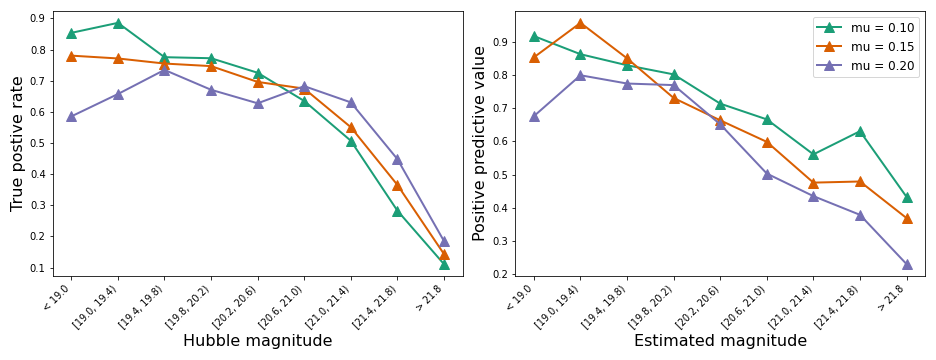
\includegraphics[width = \textwidth]{figures/prior_mu_sensitivty.png}
\end{subfigure}
\begin{subfigure}{\textwidth}
\begin{center}
\begin{tabular}{rrr}
\toprule
     mu &   TPR &   PPV \\
\midrule
 0.10 &  0.49 &  0.69 \\
 0.15 &  0.51 &  0.61 \\
 0.20 &  0.52 &  0.49 \\
\bottomrule
\end{tabular}
\par\vspace{0pt}
\end{center}
\end{subfigure}\hfill
\caption{Sensitivity of summary statistics to Poisson mean parameter on number of stars. }
\label{fig:mu_sensitivity}
\end{figure}

As $\alpha$ increases, StarNet estimates more dim sources: the prior distribution on fluxes places more mass near $f_{min}$ (Figure~\ref{fig:flux_priors}). 

\begin{figure}[!h]
    \centering
    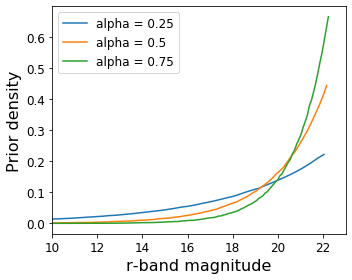
\includegraphics[width = 0.6\textwidth]{figures/prior_fluxes.png}
    \caption{The prior distribution on $r$-band magnitude for various power law slopes $\alpha$}
    \label{fig:flux_priors}
\end{figure}

While the TPR increases across $\alpha$ values, the PPV suffers at $\alpha = 0.75$ (Figure~\ref{fig:alpha_sensitivity}).
At $\alpha = 0.75$, we see that the TPR improves at dimmer sources at the expense of brighter sources, suggesting that the brigher sources become over-split. 
The stronger prior on dimmer stars also manifests in the flux distribution of the resulting StarNet catalog (Figure~\ref{fig:cdf_sensitivity}). 

\begin{figure}[ht]
\begin{subfigure}{\textwidth}
\centering
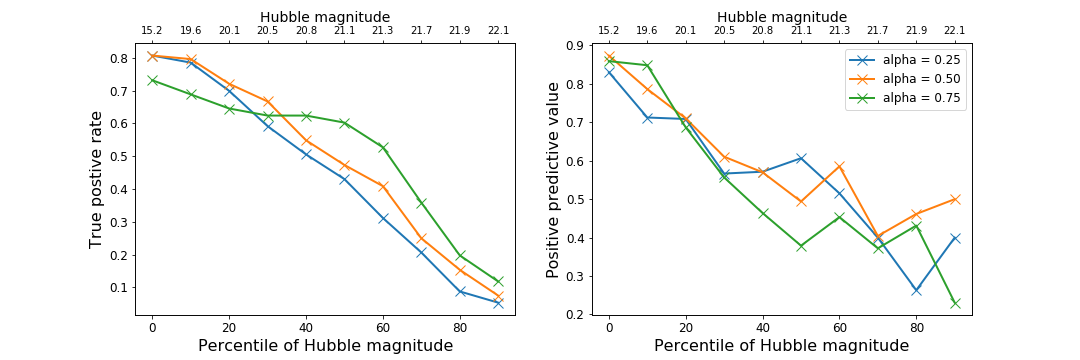
\includegraphics[width = \textwidth]{figures/prior_alpha_sensitivty.png}
\end{subfigure}
\begin{subfigure}{\textwidth}
\begin{center}
\begin{tabular}{rrr}
\toprule
 alpha &   TPR &   PPV \\
\midrule
  0.25 &  0.45 &  0.64 \\
  0.50 &  0.51 &  0.61 \\
  0.75 &  0.51 &  0.53 \\
\bottomrule
\end{tabular}
\par\vspace{0pt}
\end{center}
\end{subfigure}\hfill
\caption{Sensitivity of summary statistics to flux prior parameter $\alpha$. }
\label{fig:alpha_sensitivity}
\end{figure}

\begin{figure}
    \centering
    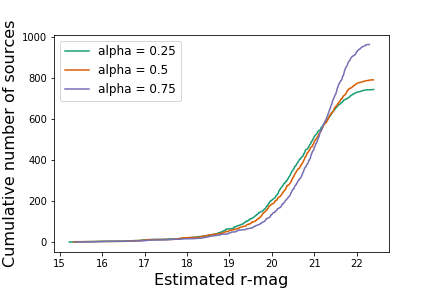
\includegraphics[width = 0.6\textwidth]{figures/sensitivity_cdf_fluxes.png}
    \caption{Sensitivity of estimated flux distribution to flux prior parameter $\alpha$}
    \label{fig:cdf_sensitivity}
\end{figure}